% \s{非磁性不純物効果を含む BCS-Legett 理論}\label{sec:form:bcsl}

ここでは、$T=0$ の超流動相における超流動秩序パラメータ $\del$ と化学ポテンシャル $\cpt$ を非磁性不純物が存在する場合に、BCS-BEC クロスオーバー全域で決定するための理論的枠組みを説明する。本研究では BCS-Leggett 理論を用いるが、実際には、有限温度の松原形式で定式化を行い、温度を十分小さくとる($T=0.01\eqf$)ことで絶対零度の計算とする(これは $\del \gg 0.01\eqf$ であれば良い近似である)。また、Nambu 表示でのハミルトニアンである式 (\ref{eq:form:ham:shkin}), (\ref{eq:form:ham:shint}), (\ref{eq:form:ham:shimp}) を用いる。

\begin{figure}[t]
\begin{center}
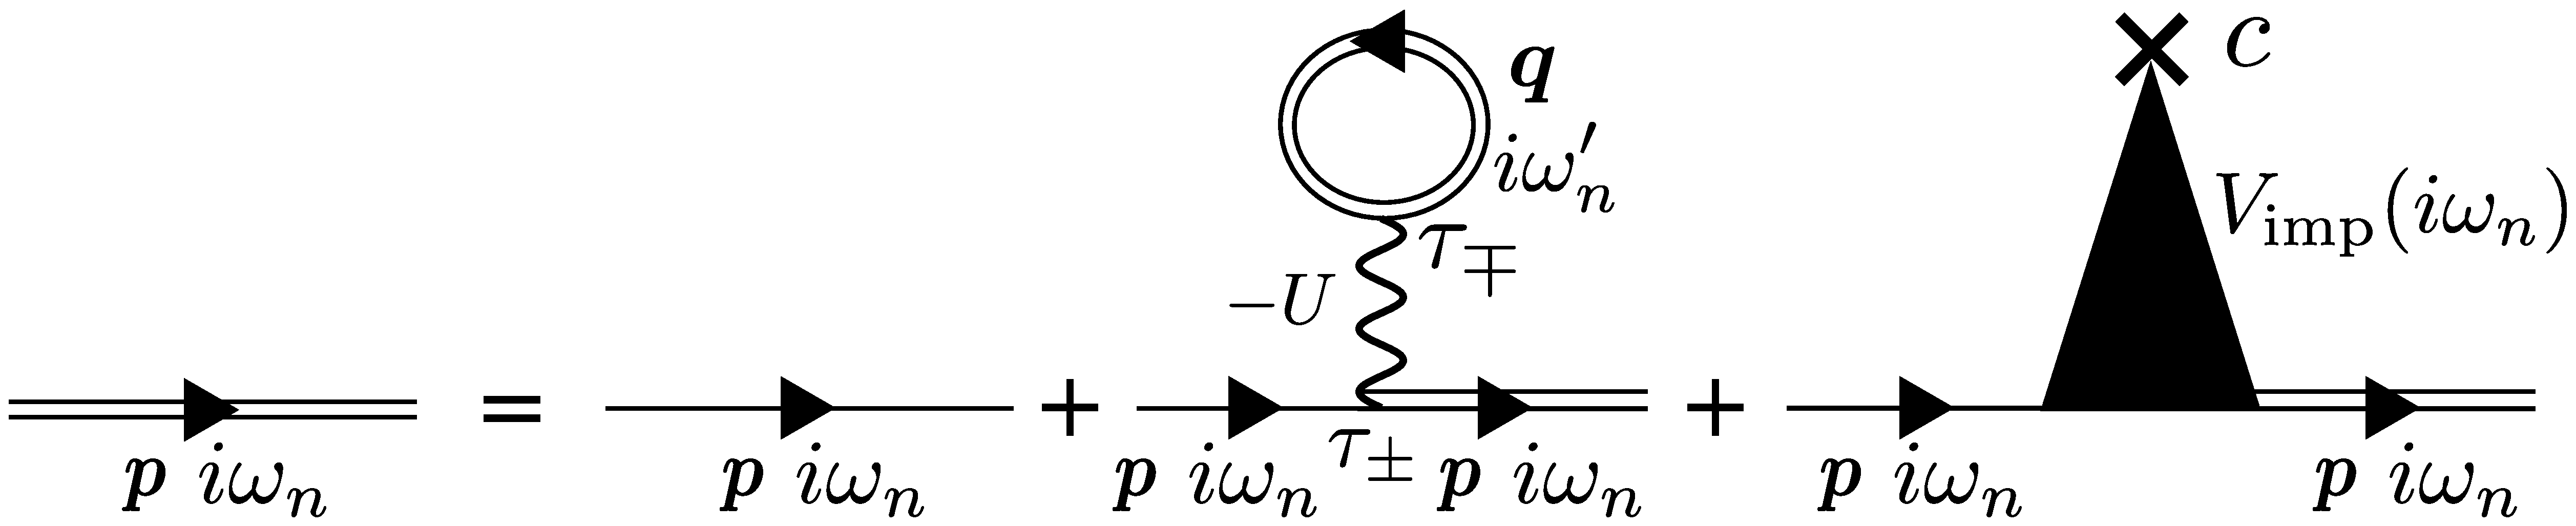
\includegraphics[width=125mm]{eps/dyson-vimp.eps}
\end{center}
\caption{非磁性不純物効果を含む BCS-Leggett 理論。実線は無摂動のグリーン関数 $\gzrpom$、二重線は全系のグリーン関数 $\bgimppom$、波線はフェッシュバッハ共鳴によるフェルミオン間相互作用 $-U$、$\times$ 印は不純物濃度 $c$、黒三角形は不純物による有効散乱強度 $\vvtxn$ を表す。}
\label{fig:form:mnf:sigimp}
\end{figure}

 1 粒子温度グリーン関数は次のダイソン方程式を満たす。
 \beq
\left[ \bgimppom \right]^{-1} = \bgzrpom^{-1} - \bsigpom.\label{eq:form:mnf:dyson0}
\eeq
ここで $\bgzrpom$ は自由フェルミ気体における Nambu 表示でのグリーン関数であり、次式で与えられる。
\beq
\bgzrpom = \frac{1}{i \omn - \left[ \ken_{\bp}- \cpt\right] \tau_3}.
\eeq

BCS-Leggett 理論の枠組みでは自己エネルギーは図 \ref{fig:form:mnf:sigimp} の右辺 1 項目と 2 項目の和で与えられ、非磁性不純物を含む場合はこれに図 \ref{fig:form:mnf:sigimp}  の最終項が加わる。

今、自己エネルギーを相互作用の寄与 $\bsigintpom$ と不純物散乱 $\bsigimppom$ に分け、
\beq
\bsigpom = \bsigintpom + \bsigimppom.\label{eq:form:mnf:sig}
\eeq
とかくと、原子間相互作用による部分は、図 \ref{fig:form:mnf:sigimp} の右辺 2 項目部分から得られ、
\beq
\bsigintpom = - \frac{U}{\beta} \sum_{\omn'} \sum_{\bpp}\left[\tau_-\Tr \left[ \tau_+ \bgimppomp  e^{i\omn'\delta}\right]+ \tau_+ \Tr \left[ \tau_- \bgimppomp  e^{i\omn'\delta}\right] \right],\label{eq:form:mnf:intpom}
\eeq
となる。超流動秩序パラメータ $\del$ は Nambu 表示のグリーン関数を用い、次のように書くことができる。
\beq
\varDelta = U \sum_{\bpp} \braket{c_{-\bpp\dar}c_{\bpp\uar}} = \frac{U}{\beta} \sum_{\omn'}\sum_{\bpp} \Tr \left[ \tau_- \bgimppomp e^{i\omn'\delta} \right].\label{eq:form:mnf:gapeq0}
\eeq
一般性を失うことなく、$\del$ が実となるように位相を選ぶと、式 (\ref{eq:form:mnf:intpom}) の自己エネルギーは次のようにまとまる。
\beq
\bsigintpom =  - \del \tau_1.\label{eq:form:mnf:delsig}
\eeq
もし不純物散乱がなければ、式 (\ref{eq:form:mnf:delsig}) を式 (\ref{eq:form:mnf:dyson0}) に代入して得られるグリーン関数、
\beq
\bgpom = \frac{1}{i\omn - \left[ \ken_{\bp} - \cpt \right]\tau_3 + \del \tau_1}
\eeq
は、Nambu 表示の下での(不純物を含まない場合の)BCS ハミルトニアン、
\beq
\hanah_{\text{BCS}} = \sum_{\bp}\varPsi_{\bp}^{\dag} \left[ \left[\ken_{\bp} - \cpt\right] \tau_3 - \del \tau_1 \vphantom{\frac{1}{2}}\right] \varPsi_{\bp},
\eeq
から得られる 1 粒子温度グリーン関数に一致する。

非磁性不純物効果を表す自己エネルギー $\bsigimppom$ は式 (\ref{eq:form:ham:abcslimp}) で与えられる自己無撞着 $T$ 行列近似の表式を用いる。こうして得られた非磁性不純物が存在する場合に拡張された BCS-Leggett 理論における 1 粒子グリーン関数は、
\beq
\bgimppom &= \frac{1}{i \omn - \left[ \ken_{\bp}- \cpt \right]\tau_3 + \del \tau_1 - \bsigimppom}\notag\\
&\equiv \frac{1}{i \tomn - \left[ \ken_{\bp} - \tcptn\right]\tau_3 + \tdeln \tau_1}.\label{eq:form:mnf:gimpopmpom}
\eeq
となる。ここで、式 (\ref{eq:form:mnf:gimpopmpom}) 2 行目は不純物散乱効果を表す自己エネルギー $\bsigimppom$ の効果を、松原周波数($\omn \to \tomn$)、超流動秩序パラメータ($\del \to \tdeln$)、および化学ポテンシャル($\cpt \to \tcptn$)にくりこんだ表式である。式 (\ref{eq:form:ham:abcslimp}) の分母について、
\beq
\sum_{\bp} \bgimppom = \sum_{\bp} \frac{1}{i\tomn - (\ken_{\bp} - \tcptn) \tau_3 + \tdeln \tau_1} = -\sum_{\bp}\frac{i\tomn - \tdeln \tau_1 + (\ken_{\bp} - \tcptn) \tau_3}{\tomn^2 + \tdeln^2 + (\ken_{\bp}-\tcptn)^2},\label{eq:form:mnf:sumg}
\eeq
と書かれることに注意すると、この表式を式 (\ref{eq:form:ham:abcslimp}) に代入した上で、式 (\ref{eq:form:mnf:gimpopmpom}) 1 行目に代入する。この式 (\ref{eq:form:mnf:gimpopmpom}) の 1 行目と 2 行目を比較して各パウリ行列の係数同士を等しいと置くことで、次の 3 つの自己無撞着方程式を得る。
\beq
\tomn &= \omn + c \frac{\frac{\tomn}{\sqrt{\tomn^2 + \tdeln^2}} \sum_{\bp} \frac{\sqrt{\tomn^2+\tdeln^2}}{\tomn^2+\tdeln^2 + (\ken_{\bp}-\tcptn)^2}}{\left[\sum_{\bp} \frac{\sqrt{\tomn^2+\tdeln^2}}{\tomn^2+\tdeln^2 + (\ken_{\bp}-\tcptn)^2}\right]^2 + \left[\frac{m}{2\pi \bs} + \sum_{\bp} \left[\frac{\ken_{\bp}-\tcptn}{\tomn^2+\tdeln^2 + (\ken_{\bp}-\tcptn)^2}- \frac{1}{\ken_{\bp}} \right]\right]^2},\label{eq:form:mnf:tomn}\\
\tdeln &=\del + c \frac{\frac{\tdeln}{\sqrt{\tomn^2 + \tdeln^2}} \sum_{\bp} \frac{\sqrt{\tomn^2+\tdeln^2}}{\tomn^2+\tdeln^2 + (\ken_{\bp}-\tcptn)^2}}{\left[\sum_{\bp} \frac{\sqrt{\tomn^2+\tdeln^2}}{\tomn^2+\tdeln^2 + (\ken_{\bp}-\tcptn)^2}\right]^2 + \left[\frac{m}{2\pi \bs} + \sum_{\bp} \left[\frac{\ken_{\bp}-\tcptn}{\tomn^2+\tdeln^2 + (\ken_{\bp}-\tcptn)^2}- \frac{1}{\ken_{\bp}} \right]\right]^2},\label{eq:form:mnf:tdeln}\\
\tcptn &=\cpt - c \frac{\frac{m}{2\pi \bs} + \sum_{\bp} \left[\frac{\ken_{\bp}-\tcptn}{\tomn^2+\tdeln^2 + (\ken_{\bp}-\tcptn)^2}- \frac{1}{\ken_p} \right]}{\left[\sum_{\bp} \frac{\sqrt{\tomn^2+\tdeln^2}}{\tomn^2+\tdeln^2 + (\ken_{\bp}-\tcptn)^2}\right]^2 + \left[\frac{m}{2\pi \bs} + \sum_{\bp} \left[\frac{\ken_{\bp}-\tcptn}{\tomn^2+\tdeln^2 + (\ken_{\bp}-\tcptn)^2}- \frac{1}{\ken_{\bp}} \right]\right]^2}.\label{eq:form:mnf:tcptn}
\eeq
式 (\ref{eq:form:mnf:tomn}), (\ref{eq:form:mnf:tdeln}), (\ref{eq:form:mnf:tcptn}) を自己無撞着に解き、($\tomn, \tdeln, \tcptn$)を決定することで、不純物効果を含む系のグリーン関数が求まる。

式 (\ref{eq:form:mnf:tomn}) の両辺を $\omn$ で割ったものと式 (\ref{eq:form:mnf:tdeln}) の両辺を $\del$ で割ったものは等しい。
\beq
\frac{\tomn}{\omn} = \frac{\tdeln}{\del}.\label{eq:form:mnf:nonmag}
\eeq
この等式を用いると、金属超伝導でよく用いられる“粒子-ホール対称性”を仮定することと、1 粒子状態密度のエネルギー依存性を無視することで、アンダーソンの定理が成立することを示すことができる(付録 \ref{sec:append:anderson} 参照)。

BCS-Leggett 理論では、$T=0$ における超流動秩序パラメータ~$\del$~と化学ポテンシャル~$\cpt$~は、ギャップ方程式 (\ref{eq:form:mnf:gapeq0}) と、粒子数方程式、
\beq
N &= \sum_{\bp,\spin} \braket{c^{\dag}_{\bp\spin}c_{\bp\spin}} = \sum_{\bp} \left[1+\braket{c^{\dag}_{\bp\uar}c_{\bp\uar}}-\braket{c_{\bp\dar}c^{\dag}_{\bp\dar}}\right]\notag\\
& =  \sum_{\bp} \left[ 1 + \frac{1}{\beta} \sumn \Tr\left[ \tau_3 \bgimppom e^{i\omn \delta}\right] \right], \label{eq:form:mnf:numeq0}
\eeq
から決定される。これらの 2 式を、式 (\ref{eq:form:mnf:tomn})-(\ref{eq:form:mnf:tcptn}) で決まる繰り込まれた変数($\tomn, \tdeln, \tcptn$)を用いて書き直すと、ギャップ方程式 (\ref{eq:form:mnf:gapeq0}) と粒子数方程式 (\ref{eq:form:mnf:numeq0}) はそれぞれ、
\beq
&\frac{m}{4 \pi \as} + \sum_{\bp}\left[ \frac{1}{\beta}\sumn \frac{ \tdeln}{\del} \frac{1}{\tomn^2+\tdeln^2 + (\ken_{\bp}-\tcptn)^2} - \frac{1}{2 \ken_{\bp}}\right] = 0, \label{eq:form:mnf:gapeq}\\
&N = \sum_{\bp} \left[ 1 - \frac{2}{\beta}\sum_n \frac{ \ken_{\bp} - \tcptn}{\tomn^2+\tdeln^2+(\ken_{\bp}-\tcptn)^2} \right], \label{eq:form:mnf:numeq}
\eeq
となる。これら 2 つの方程式と繰り込まれた量 ($\tomn, \tdeln, \tcptn$)に対する方程式 (\ref{eq:form:mnf:tomn})-(\ref{eq:form:mnf:tcptn}) を連立して解くことで不純物を含む超流動状態の BCS-BEC クロスオーバー領域における $\del$ と $\cpt$ が決定される。本研究ではこれを数値的に行う。

非磁性不純物を含まないクリーンな系の場合は($\tomn, \tdeln, \tcptn$)$\to$ ($\omn, \del, \cpt$)とすることで通常の BCS-Leggett 理論が再現される。付録 \ref{sec:append:pure:bcsl} に結果をまとめてある。

